\section{Designing a New Traffic Simulator:  Movement}

    \frame{\sectionpage}
    
    \begin{frame}{Car Movement along Edges}
        \begin{figure}
            \centering
            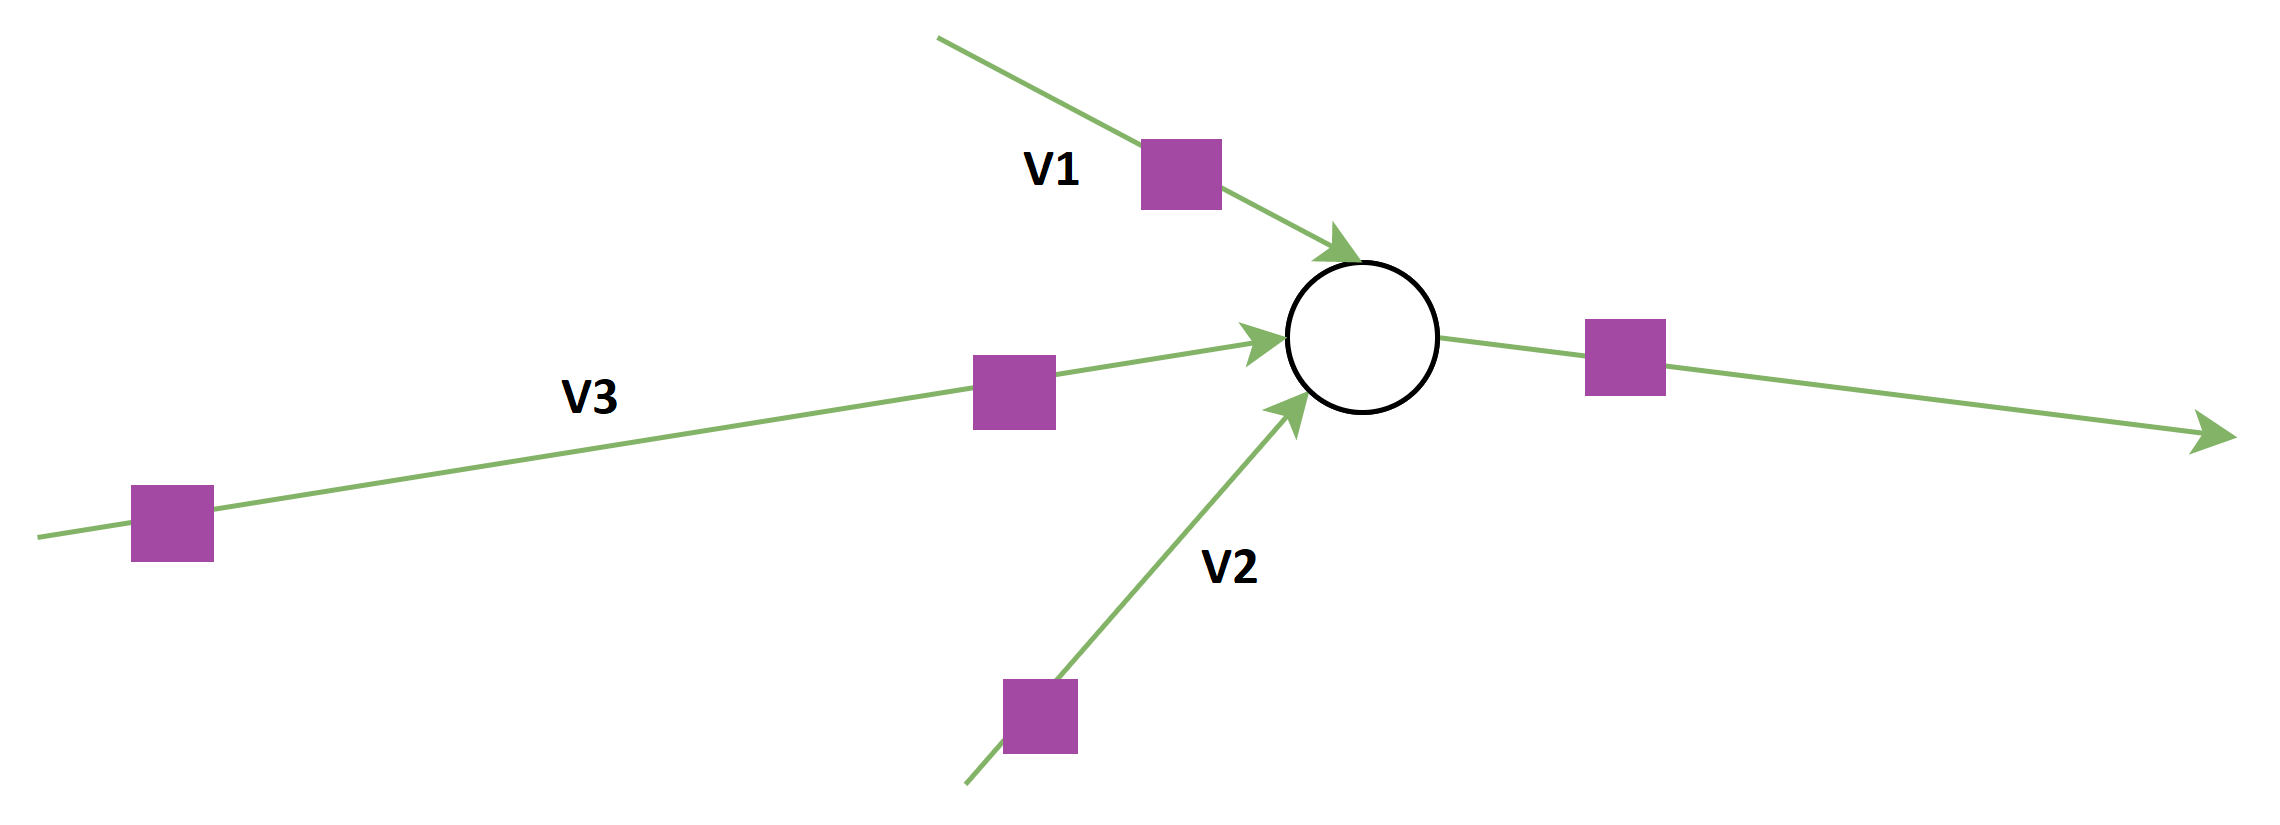
\includegraphics[height=4cm]{Images/movement_node.png}
            \caption{Several cars' positions at a moment in time}
        \end{figure}
    \end{frame}
    
    
    \begin{frame}{Movement Considerations}
        \begin{itemize}
            \item Does a car have "room" to move?
            \item How far does a car go on to the following edge?
            \item What if the two edges have different speeds?
            \item What if cars from two (or more!) different inbound edges want to move onto the same new edge?
            \item Are cars allowed to change their path?
        \end{itemize}
    \end{frame}   
    
    
    \begin{frame}{Movement Procedure}
        \begin{itemize}
            \item One unit of simulation time is a tick
            \item The entire system ticks:  \\
            TrafficManager → \textbf{|}|: Network → Node → Edge → Car :|\textbf{|}
            \item Each car per tick has a maximum "potential" energy that can be utilized to move
        \end{itemize}
    \end{frame}   
    
    \begin{frame}{What happens on a tick?}
        \begin{itemize}
            \item \textbf{TrafficManager Tick}:  tell Network to move cars as far as energy allows and advance timestamp by one tick
            \item \textbf{Network Tick}:  tell (shuffled) Nodes to tick
            \item \textbf{Node Tick}:  tell (shuffled) outbound edges to tick
            \item \textbf{Edge Tick}:  tell cars to move as much as possible***
            \item \textbf{Car Tick}:  calculate remaining potential
        \end{itemize}
    \end{frame} 
    
    \begin{frame}{Node Tick and Edge Tick}
            \begin{figure}
            \centering
            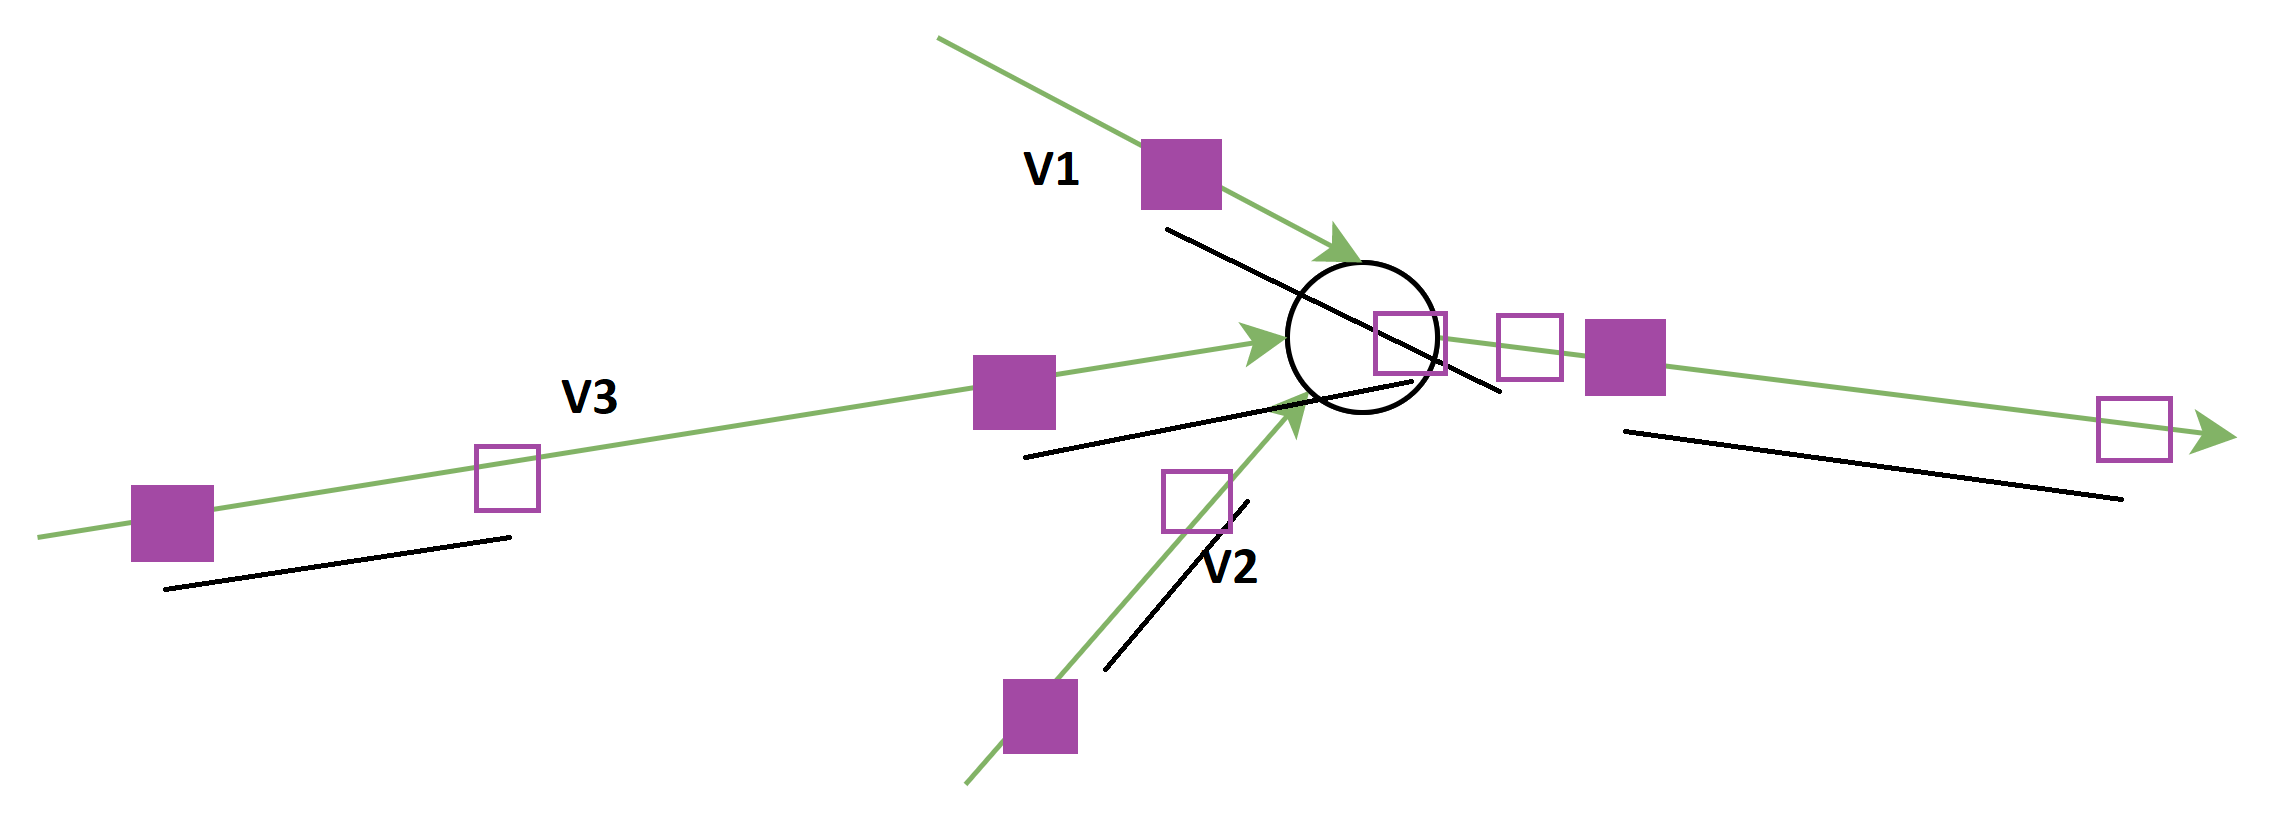
\includegraphics[height=4cm]{Images/movement_node_potentials.png}
            \caption{Eligible maximum travel distance per car has been mapped}
        \end{figure}
    \end{frame} 
    
    \begin{frame}{Node Tick}
        \begin{itemize}
            \item Check all inbound edges for cars eligible to move onto the next edge
            \item Place these eligible cars onto the start of the next edge in their path (if possible)
            \item If cars change edges, tell the old edge to forget the car and the map the car to its new edge
        \end{itemize}
    \end{frame} 
    
    \begin{frame}{Edge Tick}
        \begin{itemize}
            \item Try to move the car its maximum tick potential
            \item If it runs into another car, halt it there
            \item If it completes its route, remove it from the network
            \item If it reaches the end of the edge, wait:  it will be transfered on the next node tick
        \end{itemize}
    \end{frame} 
    
    \begin{frame}{Movement Procedure Recap}
        \begin{itemize}
            \item The entire system ticks:  \\
            TrafficManager → \textbf{|}|: Network → Node → Edge → Car :|\textbf{|}
            \item Each car per tick has a maximum "potential" energy that can be utilized to move
            \item \textbf{If no more movement is possible on the current tick, the tick is complete.  Output simulation state data.}
        \end{itemize}
    \end{frame} 